\section{Communications}\label{s:coms}
In order to control the drone, there has to be a way to transmit commands to the drone. This can be anything from simple commands like "arm motors" or complicated commands like streaming movement commands to the flight-controller on the drone.
In the following sections will different physical layers examined. 

\subsection*{Proprietary TX RX pair}\label{ss:rc-txrx}
One very common solution for radio controlled devices to communicate, is over a proprietary RF link. These systems have a remote control as the transmitter (TX) that the operator use to control the drone, and the drone then has a receiver (RX) that outputs command to the drones flight-controller.
\newline
In order to modify this signal, there are few places to break in to the signal and modify it. One could rewrite the firmware for the flight-controller, but this is out of scope for our project. Therefor another option will be used, and that option is to tap into the signal, modify it, and send the modified signal to the drone.
%This only leaves options that tap into the signal, modify it, and send the modified signal to the drone.
This can either be done in the RF signal, in the controller hardware, or between the RX and flight-controller. 

It has been chosen to tap in between the RX and flight-controller, as this is the only place to tap in, that is standardized, and the following sections will detail the protocols used here.\\
\newline

\subsection*{Drones RF specification}
In this section the RF specification for drone will be examined. 

\begin{table}[H] 
\caption{RF Specifications for communication between controller and the drone.} \label{tab:RFSpec}
\centering
\begin{tabular}{|l|m{9cm}|}
\hline
\textbf{Description}  & \textbf{Specification}                                    \\ \hline
RF range              & 2.405 - 2.475 GHz                                         \\ \hline
Channel bandwidth     & 500 KHz                                                   \\ \hline
Number of channels    & 142                                                       \\ \hline
RF power              & Less than 20 dBm                                          \\ \hline
RF mode               & AFHDS 2A (Automatic frequency hopping digital systems 2A) \\ \hline
Modulation type       & GFSK                                                      \\ \hline
Antenna length        & 26 mm * 2 (dual antenna)                                  \\ \hline
RX sensitivity        & -105 dBm                                                  \\ \hline
\end{tabular}
\end{table}

The RF specification in table \ref{tab:RFSpec} system works within 2.405 to 2.475 GHz. There are 142 channels and each channel have 500 KHz bandwidth. For each transmitter there is unique ID, when the transmitter is connected to the receiver, the receiver will save the transmitters ID, and this way the receiver will avoid other transmitter signal.
AFHDS2A, which stands for Automatic frequency hopping digital system 2A is used for radio frequency mode. This means AFHDS2A has the automatic identification function, which switches automatically in current mode between single-way communication mode and two-way communication mode. The AFHDS2A have multiple channel coding and error-correction built it. This improves the stability of the communication and reduces the error ratio and extend the reliable transmission distance. The drones transmitter and receiver specification can be found in datasheet \cite{ControllerUnit}.


\subsection*{RX protocols}\label{ss:rxprotococls} The RX connects to the flight-controller, using one or more channels, where each channel carries a control signal for a function on the drone. These channels can either be transmitted over one wire each, using PWM to express the value of the channel. Or they can all be transmitted over one wire, using PPM or other serial protocols to express the value of each channel. In both cases, the channel value is encoded in the length of a pulse. With PWM, this is the length of the high-pulse, varying from 1000 $\mu$s, to 2000 $\mu$s. The reason for using 1000 as a lower limit, is that it allows the system to tell the difference between a signal at the minimum value (1000 $\mu$s) and a missing signal (no pulse) 
An example of PWM can be seen in figure \ref{fig:chan_pwm}.

\begin{figure}[h]
    \centering
    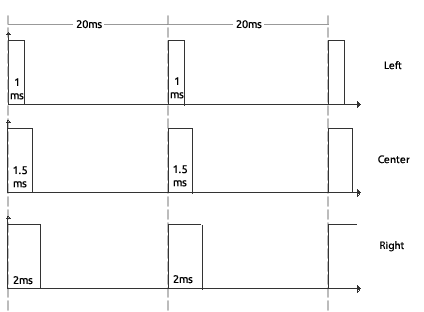
\includegraphics[width=0.7\columnwidth]{figures/PA/servo_pwm.png}
    \caption{3 Channels sent over PWM, sending the values 25\%, 75\%, and 50\% \cite{pwm-fig}.}
    \label{fig:chan_pwm}
\end{figure}

\begin{figure}[h]
    \centering
    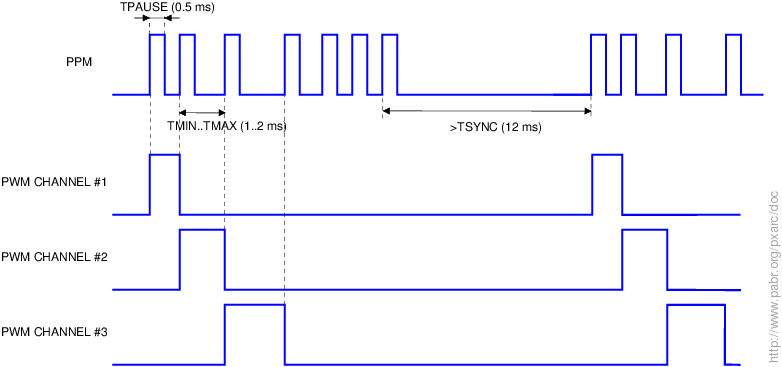
\includegraphics[width=0.8\columnwidth]{figures/PA/opwm_ppm.png}
    \caption{3 Channels sent over PPM. \cite{ppm-fig}}
    \label{fig:chan_ppm}
\end{figure}
  %\todo{Redo figure for PPM, I have no source for the current one.}
  
With PPM values are sent sequentially as seen in figure \ref{fig:chan_ppm}. Before the first channel is sent, a long "End of frame" pause is sent, holding the data-line low. This ends with a pulse, signifying start of channel1 value. Some time later, a second pulse signifies end of channel1 value, and start of channel2 value. This pattern continues until all channels have been sent, after which the "End of frame" pause is sent again.

A common problem with PWM and PPM based transmission of channel values, is that these methods encode the channel values as time between pulses of one sort or another, this means they are susceptible to jitter in the clocks on both the transmitting and receiving system.\\
In order to solve this, other serial protocols can be considered.
One such serial protocol is used internally in the receiver used on the drone. The protocol is called flySky iBUS, and is a variation of the very common RS232 serial protocol. The data-rate is fixed at 115200 baud, with 8 data bits, and 1 stop bit(8N1).

\begin{figure}[h]
    \centering
    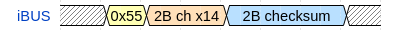
\includegraphics[width=0.8\columnwidth]{figures/ch_design/iBUS.png}
    \caption{A single iBUS packet.}
    \label{fig:iBUS}
\end{figure}

As shown on figure \ref{fig:iBUS} an iBUS packet consists of a header-byte then 28 bytes, carrying 14 16-bit values, followed by a simple 2 byte checksum. The checksum is a sum of all 14 values transmitted.

Due to the benefits that iBUS caries over PWM and PPM, this is the protocol there have been decided to further use in this project.

\subsection*{iBUS decoding and encoding}\label{iBUS library}

The code developed to decode and encode iBUS is available on github \cite{ibus-lib}.
It was written as a generic Arduino library, and this section will document key functions from it.

\begin{lstlisting}[language=C++, caption={Parser for iBUS packets.\label{lst:IBUSCL}}] 
void iBus::m_parse_channels(uint8_t packet[], int ch[])
{
	// For each channel, store 2 bytes in 16bit integer
	// The values are sent MSb first, LSB first
	for(int i=0; i<m_channels_per_packet; i++)
	{
		ch[i] = packet[i*2+2] << 8 | packet[i*2+1];
	}
}
\end{lstlisting} 

The function shown in listing \ref{lst:IBUSCL}, loops over all channel bytes in an iBUS packet, and combines them into integers in internal array to the library, a simple getter is then provided for the main program, to get individual channels.

The reverse is done to build a packet for transmitting, as seen in the following function in listing \ref{lst:PacketBuild}.

\begin{lstlisting}[language=C++, caption={Function for constructing and transmitting for iBUS packets. \label{lst:PacketBuild}}]
void iBus::m_send_packet(int ch[])
{
	// Set up buffer and set header byte
	uint8_t buff[m_packet_size];
	buff[0] = 0x55;

	// For each channel, unpack 16 bit integer into bytes
	// The values are sent MSb first, LSB first.
	for(int i=0; i<m_channels_per_packet; i++)
	{
		buff[i*2+1] = (ch[i] & 0x00FF);
		buff[i*2+2] = (ch[i] >> 8);
	}
	int checksum = m_get_checksum(ch);

	buff[29] = (checksum & 0x00FF);
	buff[30] = (checksum >> 8);

	m_ser.write(buff, m_packet_size);
}
\end{lstlisting}

As seen in listing \ref{lst:PacketBuild} this function, constructing and sending an iBUS package. %is rather simple.
The code allocates a buffer to hold a packet, sets the header-byte, and then splits apart the 14 channels supplied into individual bytes, arranged Most Significant Bit (MSb), Less Significant Byte (LSB) first. This means a number such as 0x0102 would be sent as 0x02, 0x01. From here, the checksum is calculated, split into the same MSb, LSB first arrangement, and the whole buffer is written out over the allocated stream object \textbf{\textit{m\_ser}}.

The function used to set which channel values are sent, is a simple setter function. Setting the values of an internal output channel array, which is passed to \textbf{\textit{m\_send\_packet\(\)}} each time the main ticker function \textbf{\textit{handle\(\)}} is called.

The handle function is more easily described with a flow-chart, as it is a relatively long function. The flow-chart can be seen in figure \ref{fig:ibus_handle_flowchart}.

\begin{figure}[h]
    \centering
    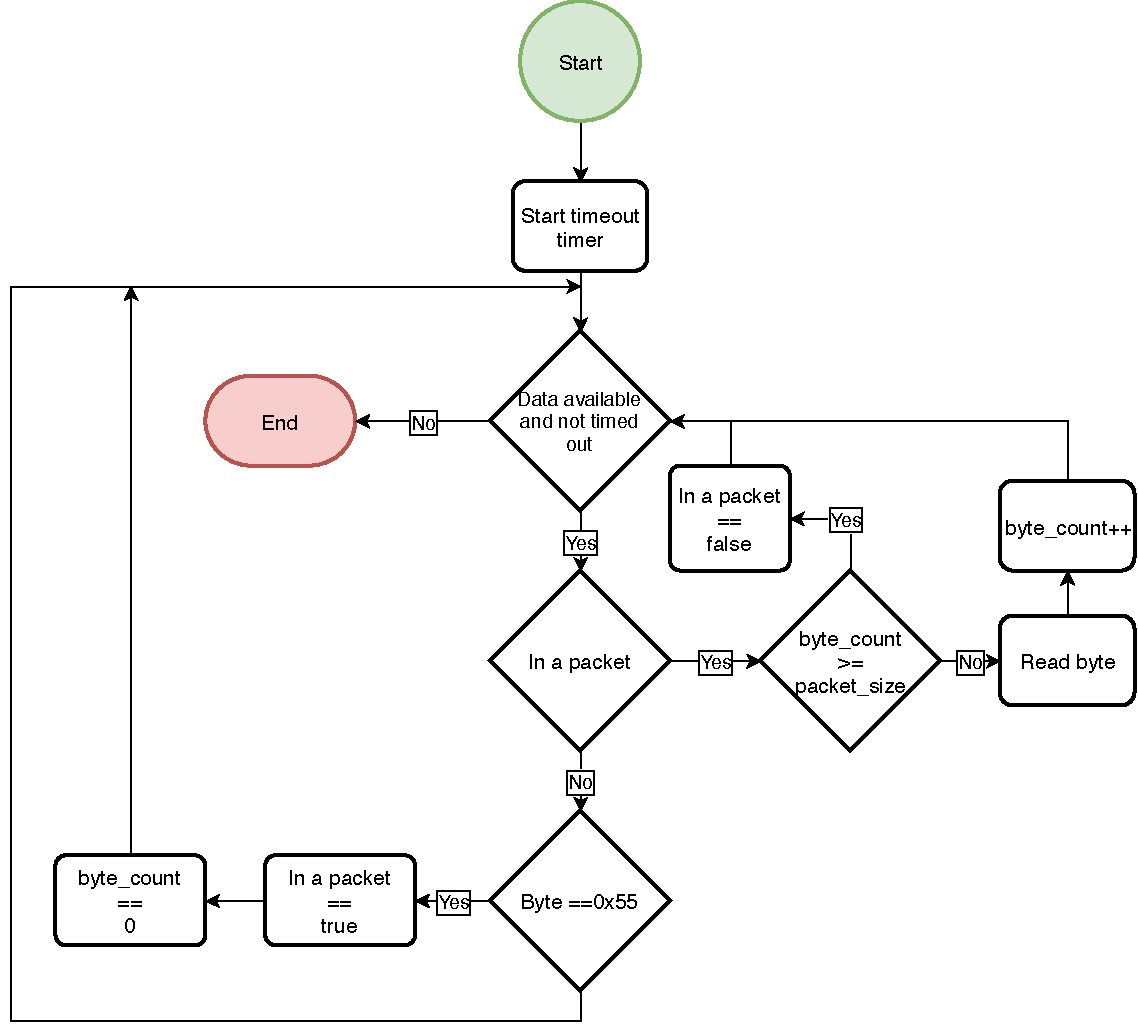
\includegraphics[width=\columnwidth]{figures/ch_design/ibus-handle-flowchart.pdf}
    \caption{Flowchart describing the handle function in the iBUS library.}
    \label{fig:ibus_handle_flowchart}
\end{figure}

